\documentclass[border=10pt]{standalone}

\usepackage{tikz}
\usepackage{tikzsymbols}
\usetikzlibrary{calc,patterns,shapes.geometric}

\def\centerarc[#1](#2)(#3:#4:#5){\draw[#1] ($(#2)+({#5*cos(#3)},{#5*sin(#3)})$) arc (#3:#4:#5);}

\begin{document}
	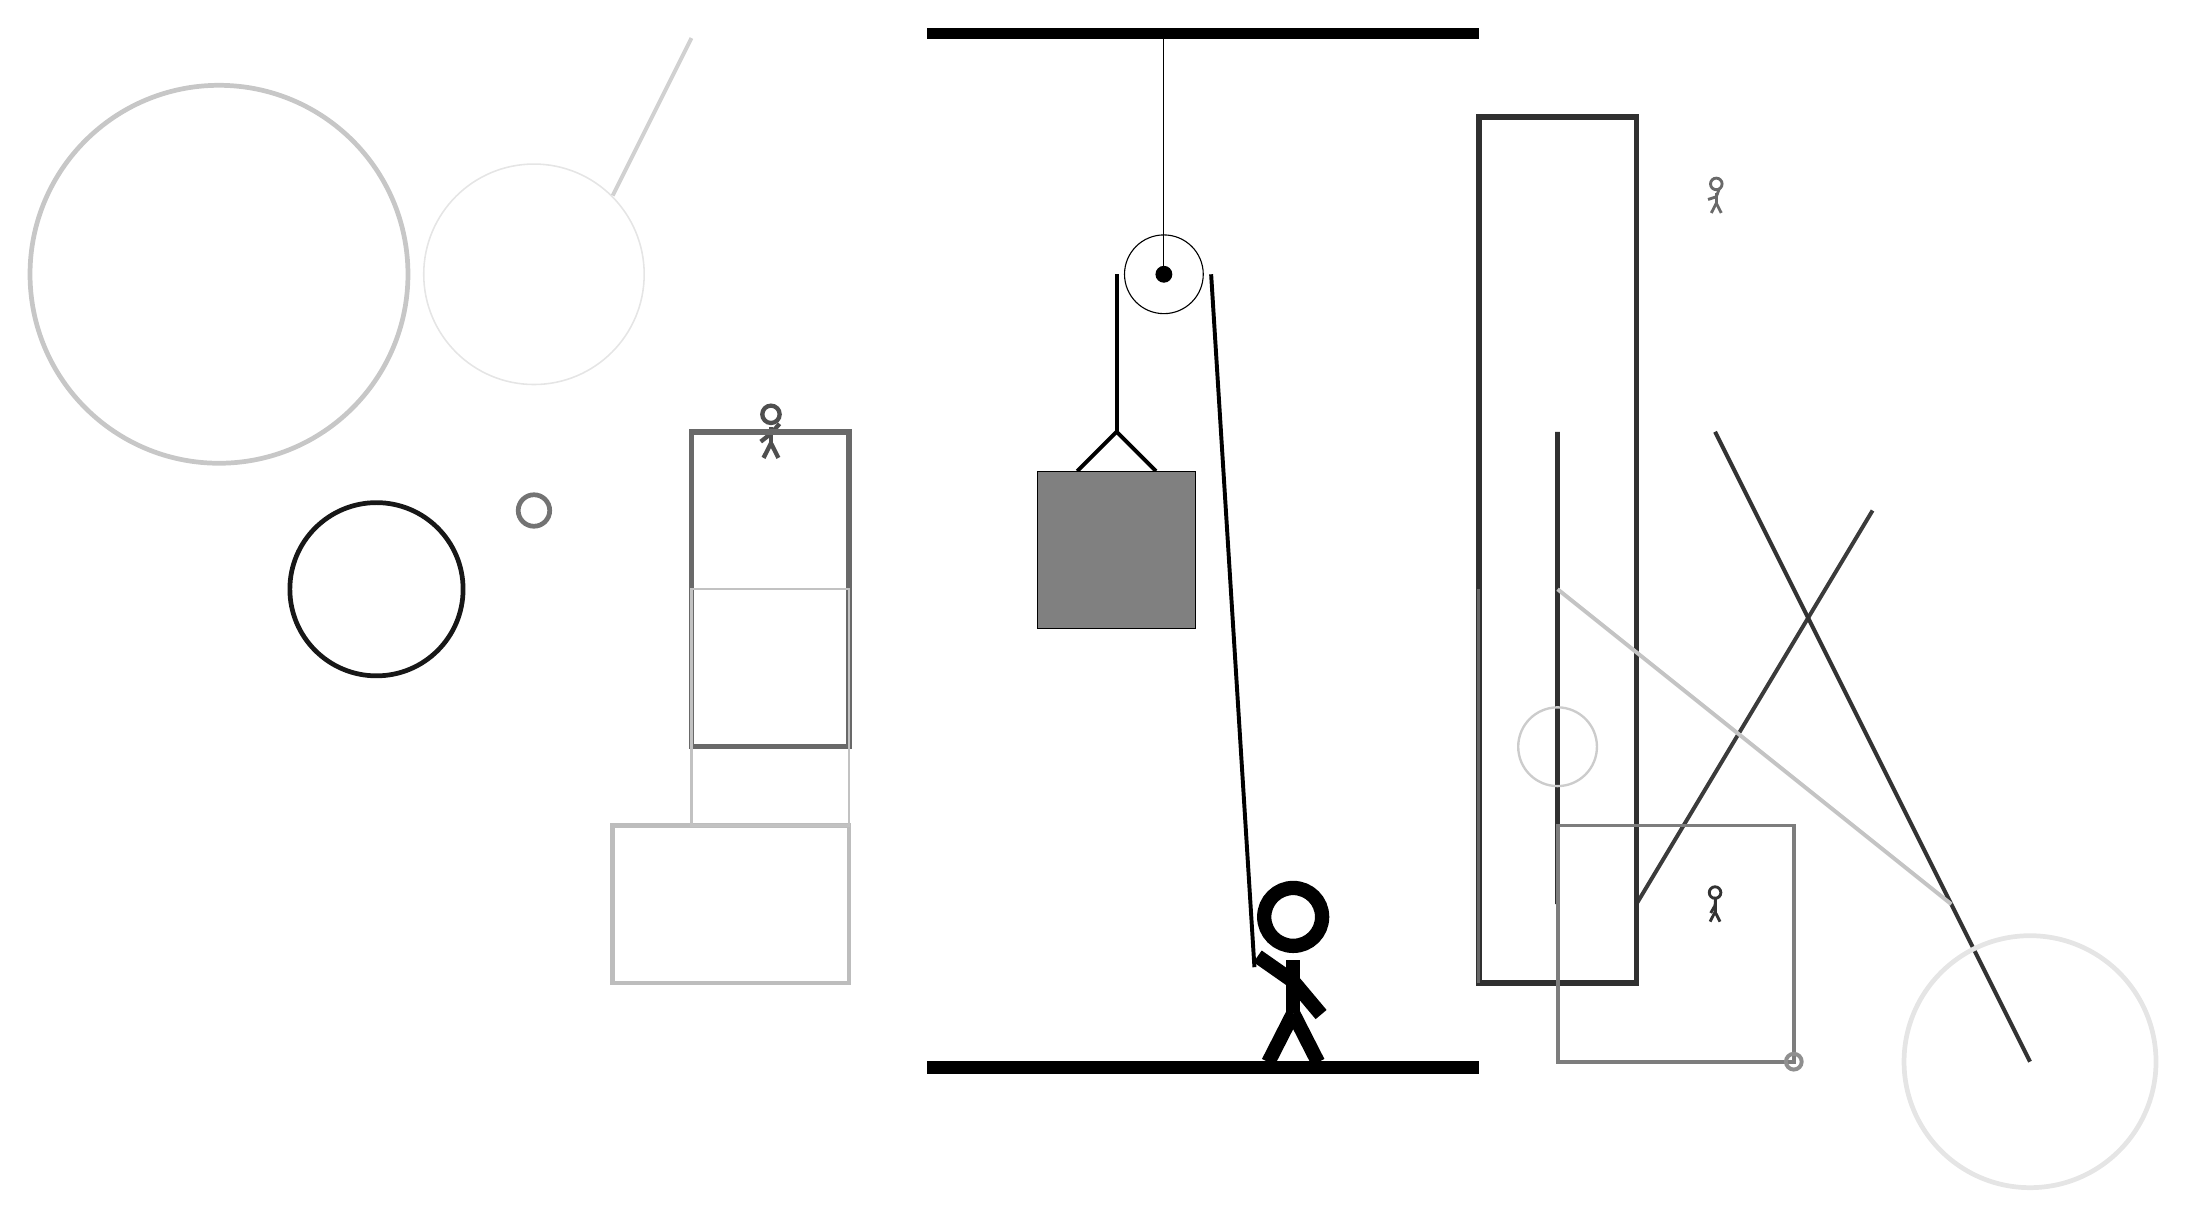
\begin{tikzpicture}
		%%%%% START %%%%%
		
		\draw[fill=black] (-2, 10) rectangle (5, 10.125);
		
		\draw (1, 7) circle (0.5);
		\draw[fill=black] (1, 7) circle (0.1);
		\draw (1, 10) -- (1, 7);
		
		\draw[line width=0.5mm] (-0.1, 4.5) -- (0.4, 5.0) -- (0.9, 4.5);
		\draw[fill=black!50] (-0.6, 4.5) rectangle (1.4, 2.5);
		
		\draw[line width=0.5mm] (0.4, 7) -- (0.4, 5.0);
		\centerarc[line width=0.5mm](1, 7)(0:180:0.6);
		\draw[line width=0.5mm](1.6, 7) -- (2.15, -1.8);
		
		\draw[line width=0.7mm, color=black!81] (6, -1) rectangle (6, 5);
		
		\draw [line width=0.6mm, color=black!55](-7, 4) circle (0.2);
		\draw[line width=0.5mm, color=black!77](7, -1) -- (10, 4);
		\draw[line width=0.7mm, color=black!81] (7, 9) rectangle (5, -2);
		\draw[line width=0.5mm, color=black!80](8, 5) -- (12, -3);
		\node[line width=0.2mm, color=black!69] at (-4, 5) {\Strichmaxerl[3][38][49]};
		\draw[line width=0.7mm, color=black!59] (-3, 1) rectangle (-5, 5);
		\draw [line width=0.2mm, color=black!10](-7, 7) circle (1.4);
		\draw [line width=0.6mm, color=black!10](12, -3) circle (1.6);
		\node[line width=0.6mm, color=black!59] at (8, 8) {\Strichmaxerl[2][18][70]};
		
		\draw[line width=0.5mm, color=black!51] (6, -3) rectangle (9, 0);
		
		\draw [line width=0.5mm, color=black!44](9, -3) circle (0.1);
		\draw [line width=0.3mm, color=black!20](6, 1) circle (0.5);
		\draw [line width=0.6mm, color=black!22](-11, 7) circle (2.4);
		\draw[line width=0.5mm, color=black!23](6, 3) -- (11, -1);
		\draw[line width=0.6mm, color=black!26] (-3, 0) rectangle (-6, -2);
		\draw[line width=0.4mm, color=black!60] (5, 3) rectangle (5, -2);
		\draw[line width=0.3mm, color=black!24] (-3, 0) rectangle (-5, 3);
		\draw[line width=0.5mm, color=black!18](-5, 10) -- (-6, 8);
		\draw [line width=0.6mm, color=black!91](-9, 3) circle (1.1);
		\node[line width=0.2mm, color=black!80] at (8, -1) {\Strichmaxerl[2][60][86]};
		
		
		\node at (2.6, -1.9) {\Strichmaxerl[10][-35][-50]};
		
		\draw[fill=black] (-2, -3) rectangle (5, -3.15);
		
		%%%%% END %%%%%
	\end{tikzpicture}
\end{document}